\documentclass[tikz,border=1mm]{standalone}
\usepackage[T1]{fontenc}
\usepackage{lmodern}
\usepackage{amsmath}
\usetikzlibrary{arrows.meta,patterns}
\definecolor{navy}{HTML}{17486D}
\definecolor{teal}{HTML}{145B54}
\definecolor{slate}{HTML}{354758}
\definecolor{rust}{HTML}{A14633}

\begin{document}
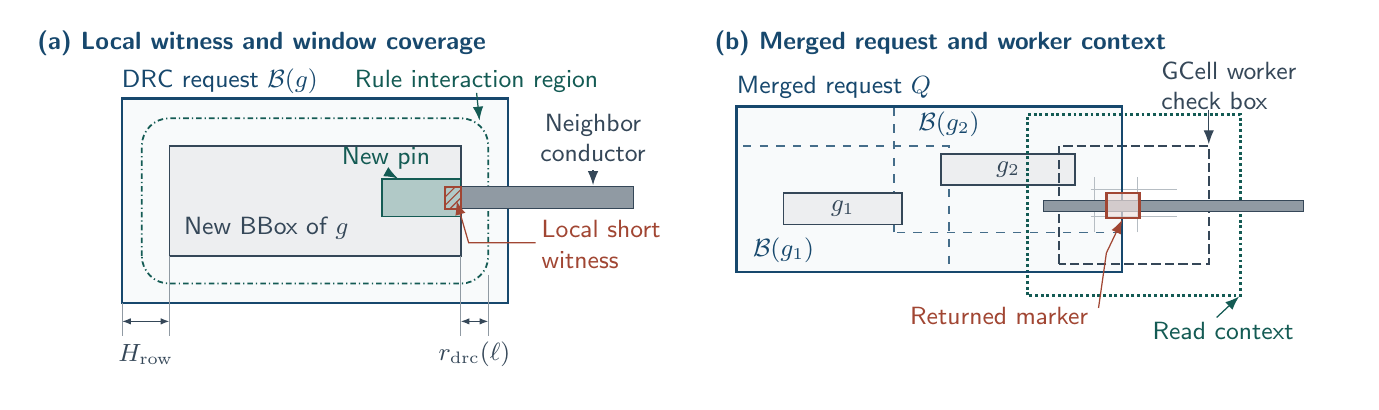
\begin{tikzpicture}[
  x=1mm,y=1mm,font=\sffamily\small,>=Latex,
  request/.style={draw=navy,line width=.85pt},
  cell/.style={draw=slate,line width=.65pt,fill=slate!9},
  conductor/.style={draw=slate,fill=slate!55,line width=.35pt},
  leader/.style={-Latex,draw=slate,line width=.45pt,shorten >=.2mm},
  guide/.style={draw=slate!55,line width=.35pt},
  measure/.style={{Latex[length=1.1mm]}-{Latex[length=1.1mm]},draw=slate,line width=.45pt}
]
\path[use as bounding box] (0,0) rectangle (168,45);

% (a) Local geometric witness. The pin touches the right edge of the new
% instance BBox; only its positive-area intersection with the long conductor
% is shaded as the witness.
\node[anchor=west,font=\sffamily\bfseries\small,text=navy] at (0,43)
  {(a) Local witness and window coverage};
\fill[navy!3] (12,10) rectangle (61,36);
\draw[request] (12,10) rectangle (61,36);
\draw[teal,dash pattern=on 2pt off 1.1pt on .45pt off 1.1pt,line width=.65pt,
      rounded corners=3.5mm] (14.5,12.5) rectangle (58.5,33.5);
\draw[cell] (18,16) rectangle (55,30);
\draw[conductor] (53,22) rectangle (77,24.8);
\draw[teal,fill=teal!33,line width=.5pt] (45,21) rectangle (55,25.8);
\fill[pattern=north east lines,pattern color=rust] (53,22) rectangle (55,24.8);
\draw[rust,line width=.75pt] (53,22) rectangle (55,24.8);

\node[anchor=west,text=navy,inner sep=0pt] at (11.9,38.2)
  {DRC request \(\mathcal B(g)\)};
\node[anchor=west,text=teal,inner sep=0pt] (halo) at (41.5,38.2)
  {Rule interaction region};
\draw[leader,draw=teal] (halo.south) -- (57.4,33);
\node[anchor=west,text=slate,inner sep=0pt] at (19.8,19.5)
  {New BBox of \(g\)};
\node[anchor=south,text=teal,inner sep=0pt] at (45.5,26.9) {New pin};
\draw[leader,draw=teal] (45.5,26.7) -- (47.2,25.75);
\node[align=center,text=slate,inner sep=0pt] at (71.8,31) {Neighbor\\conductor};
\draw[leader] (71.8,26.9) -- (71.8,24.8);
\node[anchor=west,align=left,text=rust,inner sep=0pt] at (65.2,17.5)
  {Local short\\witness};
\draw[leader,draw=rust] (64.5,17.7) -- (56,17.7) -- (54.4,23.2);

\draw[guide] (12,10) -- (12,5.8) (18,16) -- (18,5.8)
             (55,16) -- (55,5.8) (58.5,13.6) -- (58.5,5.8);
\draw[measure] (12,7.7) -- (18,7.7);
\draw[measure] (55,7.7) -- (58.5,7.7);
\node[text=slate,inner sep=0pt] at (15,3.5) {\(H_{\mathrm{row}}\)};
\node[text=slate,inner sep=0pt] at (56.75,3.5) {\(r_{\mathrm{drc}}(\ell)\)};

% (b) The solid request is the enclosing rectangle of two overlapping seed
% windows. Coincident exterior edges belong to both the seed and merged boxes;
% the dashed interior segments retain their individual outlines.
\begin{scope}[shift={(86,0)}]
\node[anchor=west,font=\sffamily\bfseries\small,text=navy] at (0,43)
  {(b) Merged request and worker context};
\fill[navy!3] (4,14) rectangle (53,35);
\draw[navy!80,dashed,line width=.55pt] (4,14) rectangle (31,30);
\draw[navy!80,dashed,line width=.55pt] (24,19) rectangle (53,35);
\draw[cell] (10,20) rectangle (25,24);
\draw[cell] (30,25) rectangle (47,29);
\node[text=slate,inner sep=0pt] at (17.5,22) {\(g_1\)};
\node[text=slate,inner sep=0pt] at (38.5,27) {\(g_2\)};
\node[text=navy,inner sep=0pt] at (10,16.7) {\(\mathcal B(g_1)\)};
\node[text=navy,inner sep=0pt] at (31,32.7) {\(\mathcal B(g_2)\)};

\draw[teal,densely dotted,line width=1.05pt] (41,11) rectangle (68,34);
\draw[slate,dash pattern=on 3.4pt off 1.5pt,line width=.7pt]
  (45,15) rectangle (64,30);
\draw[slate!36,line width=.35pt] (49,19) grid[xstep=5.5,ystep=3.5] (60,26);
\draw[request] (4,14) rectangle (53,35);
\draw[conductor] (43,21.7) rectangle (76,23.1);
\draw[rust,fill=rust!16,fill opacity=.7,line width=.85pt]
  (51,20.8) rectangle (55.2,24);
\node[anchor=west,text=navy,inner sep=0pt] at (4,37.4) {Merged request \(Q\)};
\node[anchor=west,align=left,text=slate,inner sep=0pt] at (57.9,37.6)
  {GCell worker\\check box};
\draw[leader] (64,34.5) -- (64,30);
\node[anchor=west,text=rust,inner sep=0pt] at (26,8.4) {Returned marker};
\draw[leader,draw=rust] (50,9.4) -- (51,16.4) -- (53.1,20.8);
\node[anchor=west,text=teal,inner sep=0pt] at (56.8,6.5) {Read context};
\draw[leader,draw=teal] (65,8.2) -- (68,11);
\end{scope}
\end{tikzpicture}
\end{document}
